\chapter{Ap\'endice}

\section{Escenarios de \textit{policy iteration}}

En este apartado se recopilan escenarios probados para el algoritmo \textit{Policy Iteration}. Tales escenarios constituyen, en su mayor\'ia, cambios en las condiciones iniciales del mundo, para visualizar los efectos en las estrategias aprendidas.\\

El escenario A muestra los resultados al iniciar uno de los agentes, en este caso el almac\'en regional, con un inventario de $500$ unidades, mientras que los dem\'as comienzan con $10$ unidades. Se puede observar que los agentes inferiores al almac\'en reconocen que hay existencias, y entonces su cantidad demandada es mayor a cero hasta el momento en el que el inventario del almac\'en se termina. Por otro lado, ni el almac\'en ni la f\'abrica presentan demanda constantemente positiva al principio del a\~no, pues ellos no pueden tomar decisiones diferentes en ese periodo debido la inyecci\'on de inventario.\\

Para el escenario B, se utiliz\'o una tendencia de producci\'on en los campos diferente de la utilizada en todo el trabajo, para demostrar que los agentes aprender\'an nuevas tendencias en caso de que estas cambien. Los nuevos valores fueron creados manualmente sin ninguna l\'ogica espec\'ifica. Puede notarse que todos los agentes cambian sus pol\'iticas \'optimas para comprar cuando hay producci\'on en los campos. \\

\begin{figure}[H]
\caption{Escenario A}
\label{scen_wholesale_500}
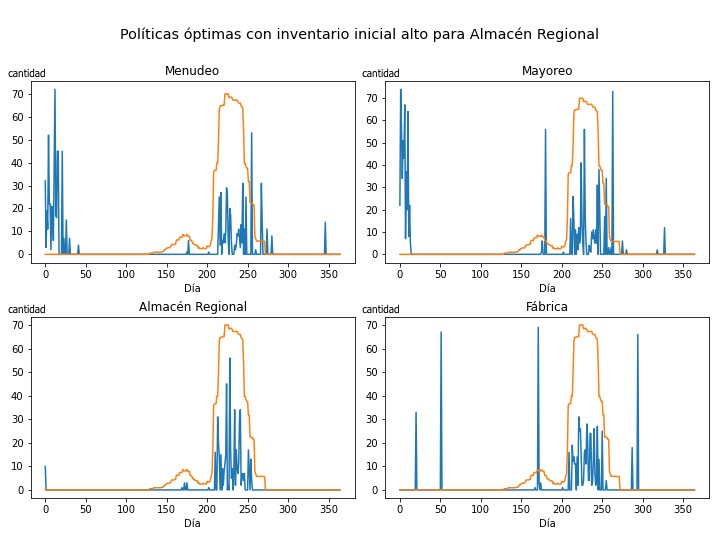
\includegraphics[width=9cm]{tesis_tex/figs/policyiteration_scen_wholesale500.png}
\centering
\end{figure}

\begin{figure}[H]
\caption{Escenario B}
\label{scen_alternative_supply}
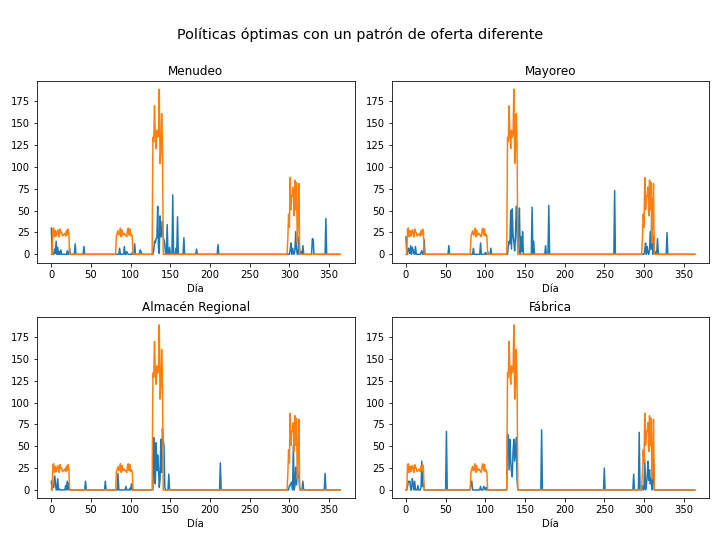
\includegraphics[width=9cm]{tesis_tex/figs/policyiteration_scen_alternativesupply.png}
\centering
\end{figure}